\documentclass[french, utf8]{article}
\usepackage[utf8]{inputenc}
\usepackage[T1]{fontenc}
\usepackage[french]{babel}
\usepackage[parfill]{parskip}
\usepackage{amsmath}
\usepackage{amssymb}
\usepackage{amsfonts}
\usepackage{graphicx}
\usepackage{subfigure}
\usepackage[font={small}]{caption}
\usepackage{float}
\usepackage{listingsutf8}
\usepackage{fullpage}
\usepackage[nochapter]{vhistory}
\usepackage{hyperref}
\usepackage{titlesec}
\usepackage{xcolor}
\usepackage{verbatim}
\usepackage{graphicx}
\usepackage{listings}
\usepackage{subcaption}
\usepackage{comment}
%\usepackage[export]{adjustbox}
\usepackage{adjustbox}

\begin{comment}
\usepackage{xcolor,colortbl}

\newcommand{\mc}[2]{\multicolumn{#1}{c}{#2}}
\definecolor{Gray}{gray}{0.85}
\definecolor{LightCyan}{rgb}{0.88,1,1}

\newcolumntype{grey}{>{\columncolor{Gray}}c}
\newcolumntype{white}{>{\columncolor{white}}c}

\end{comment}


\newcommand*{\MyIncludeGraphicsMaxSize}[2][]{%
\begin{adjustbox}{max size={\textwidth}{\textheight}}
    \includegraphics[#1]{#2}%
\end{adjustbox}
}

\usepackage{array,booktabs,ragged2e}
\newcolumntype{R}[1]{>{\RaggedLeft\arraybackslash}p{#1}}
\newcolumntype{D}[1]{>{\RaggedLeft\arraybackslash}p{#1}}

%\usepackage{listingsutf8}


\title{INFO-H303 - Projet bases de données - ATASCO}
\author{Bourgeois Noé (000496667) & Moruntale Vlad (000515147) & Aguililla Klein Esteban(000514341) }
\date{Mars 2022}

\begin{document}

%\lstset{inputencoding=utf8/latin1}

\maketitle

\tableofcontents

\newpage

\section{Introduction}
cf énoncé:
"L’Air Travel Association for Statistics, Computing and Optimization (ATASCO) a reçu des données de différentes compagnies aériennes US, avec l’objectif d’aider ces compagnies à améliorer leurs offres et réduire leurs coûts.
L’association doit créer une base de données. La 1ère étape consiste à créer un modèle entité-association ainsi qu’un modèle relationnel."


\section[Diagramme entité-association]{Diagramme entité-association \footnote{"Le modèle entité-association (EA) (le terme « entité-relation » est une traduction erronée largement répandue), ou diagramme entité-association ou en anglais « entity-relationship diagram », abrégé en ERD" voir section \ref{sec:ref}}}

\begin{figure}[h]
    \centering
    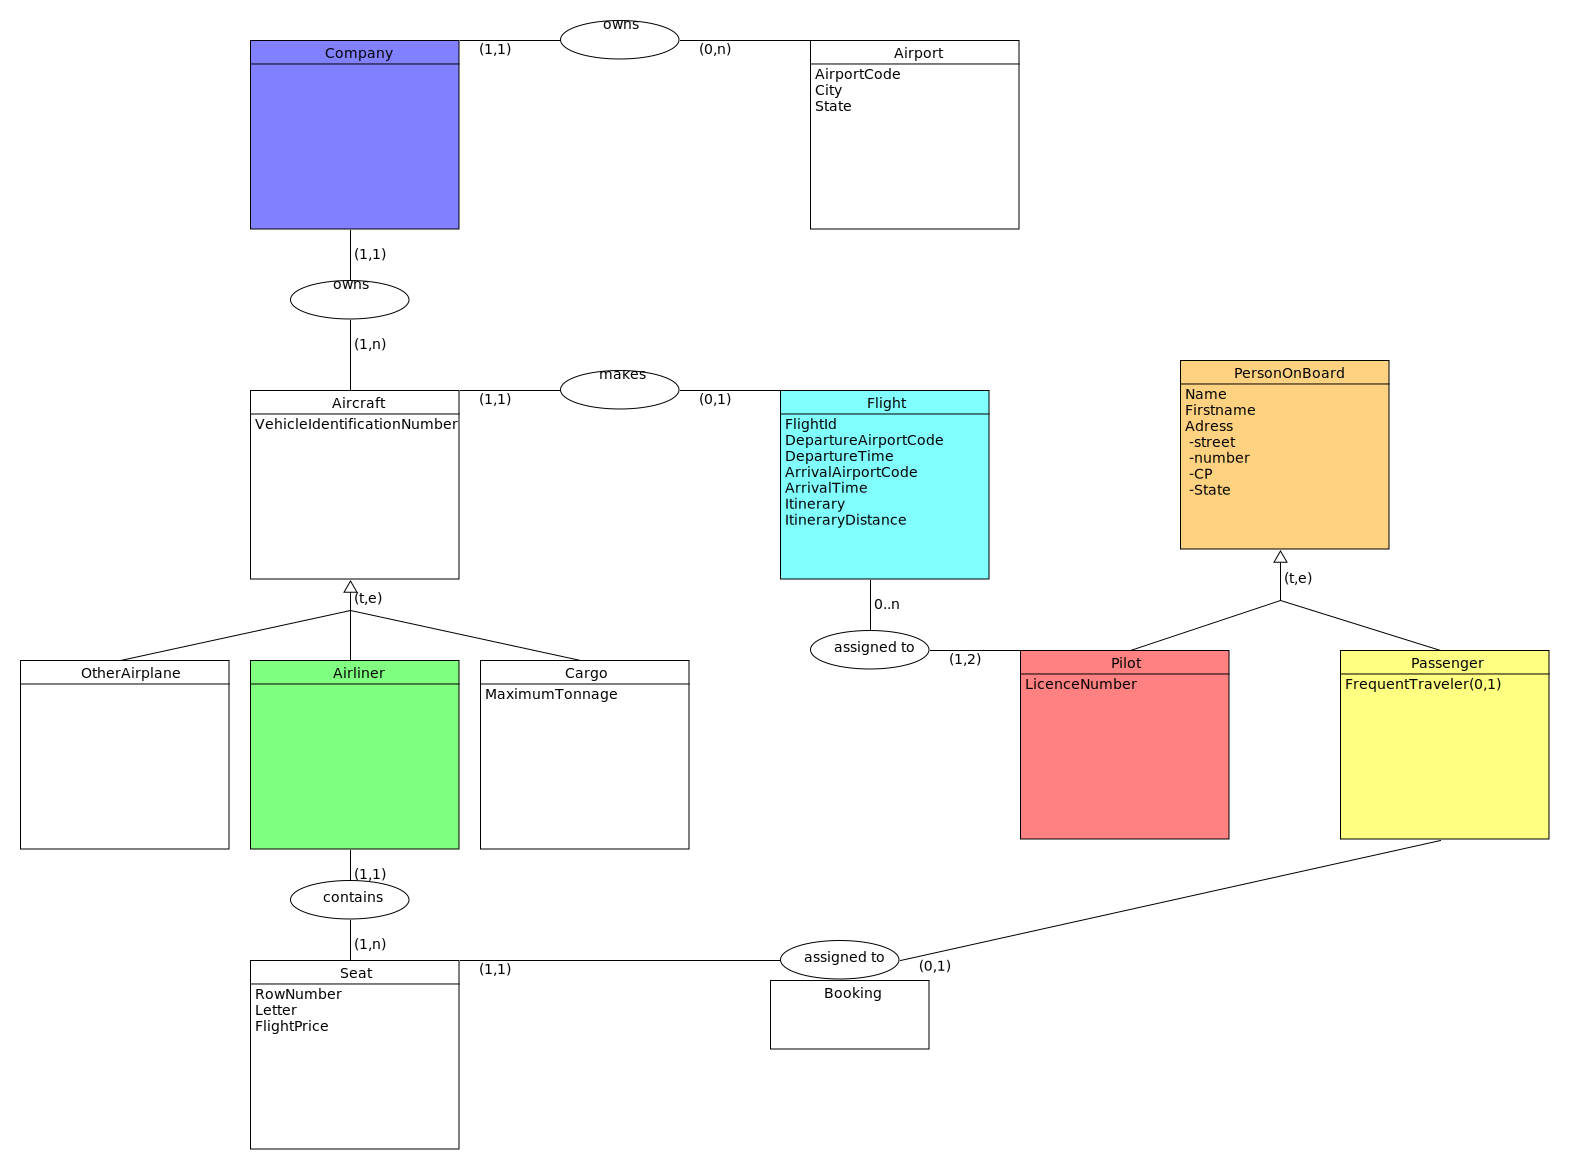
\includegraphics[width=\textwidth]{image/ATASCO-entity-relationship-diagram.png}
    \caption{Diagramme entité-association partie 1 }
    \label{fig:diag_p1}
\end{figure}

\newpage<


\begin{figure}[h]
    \centering
    \includegraphics[scale=0.6]{image/correction.png}
    \caption{Diagramme entité-association correction}
    \label{fig:diag_correction}
\end{figure}

\newpage


\begin{figure}[h]
    \centering
    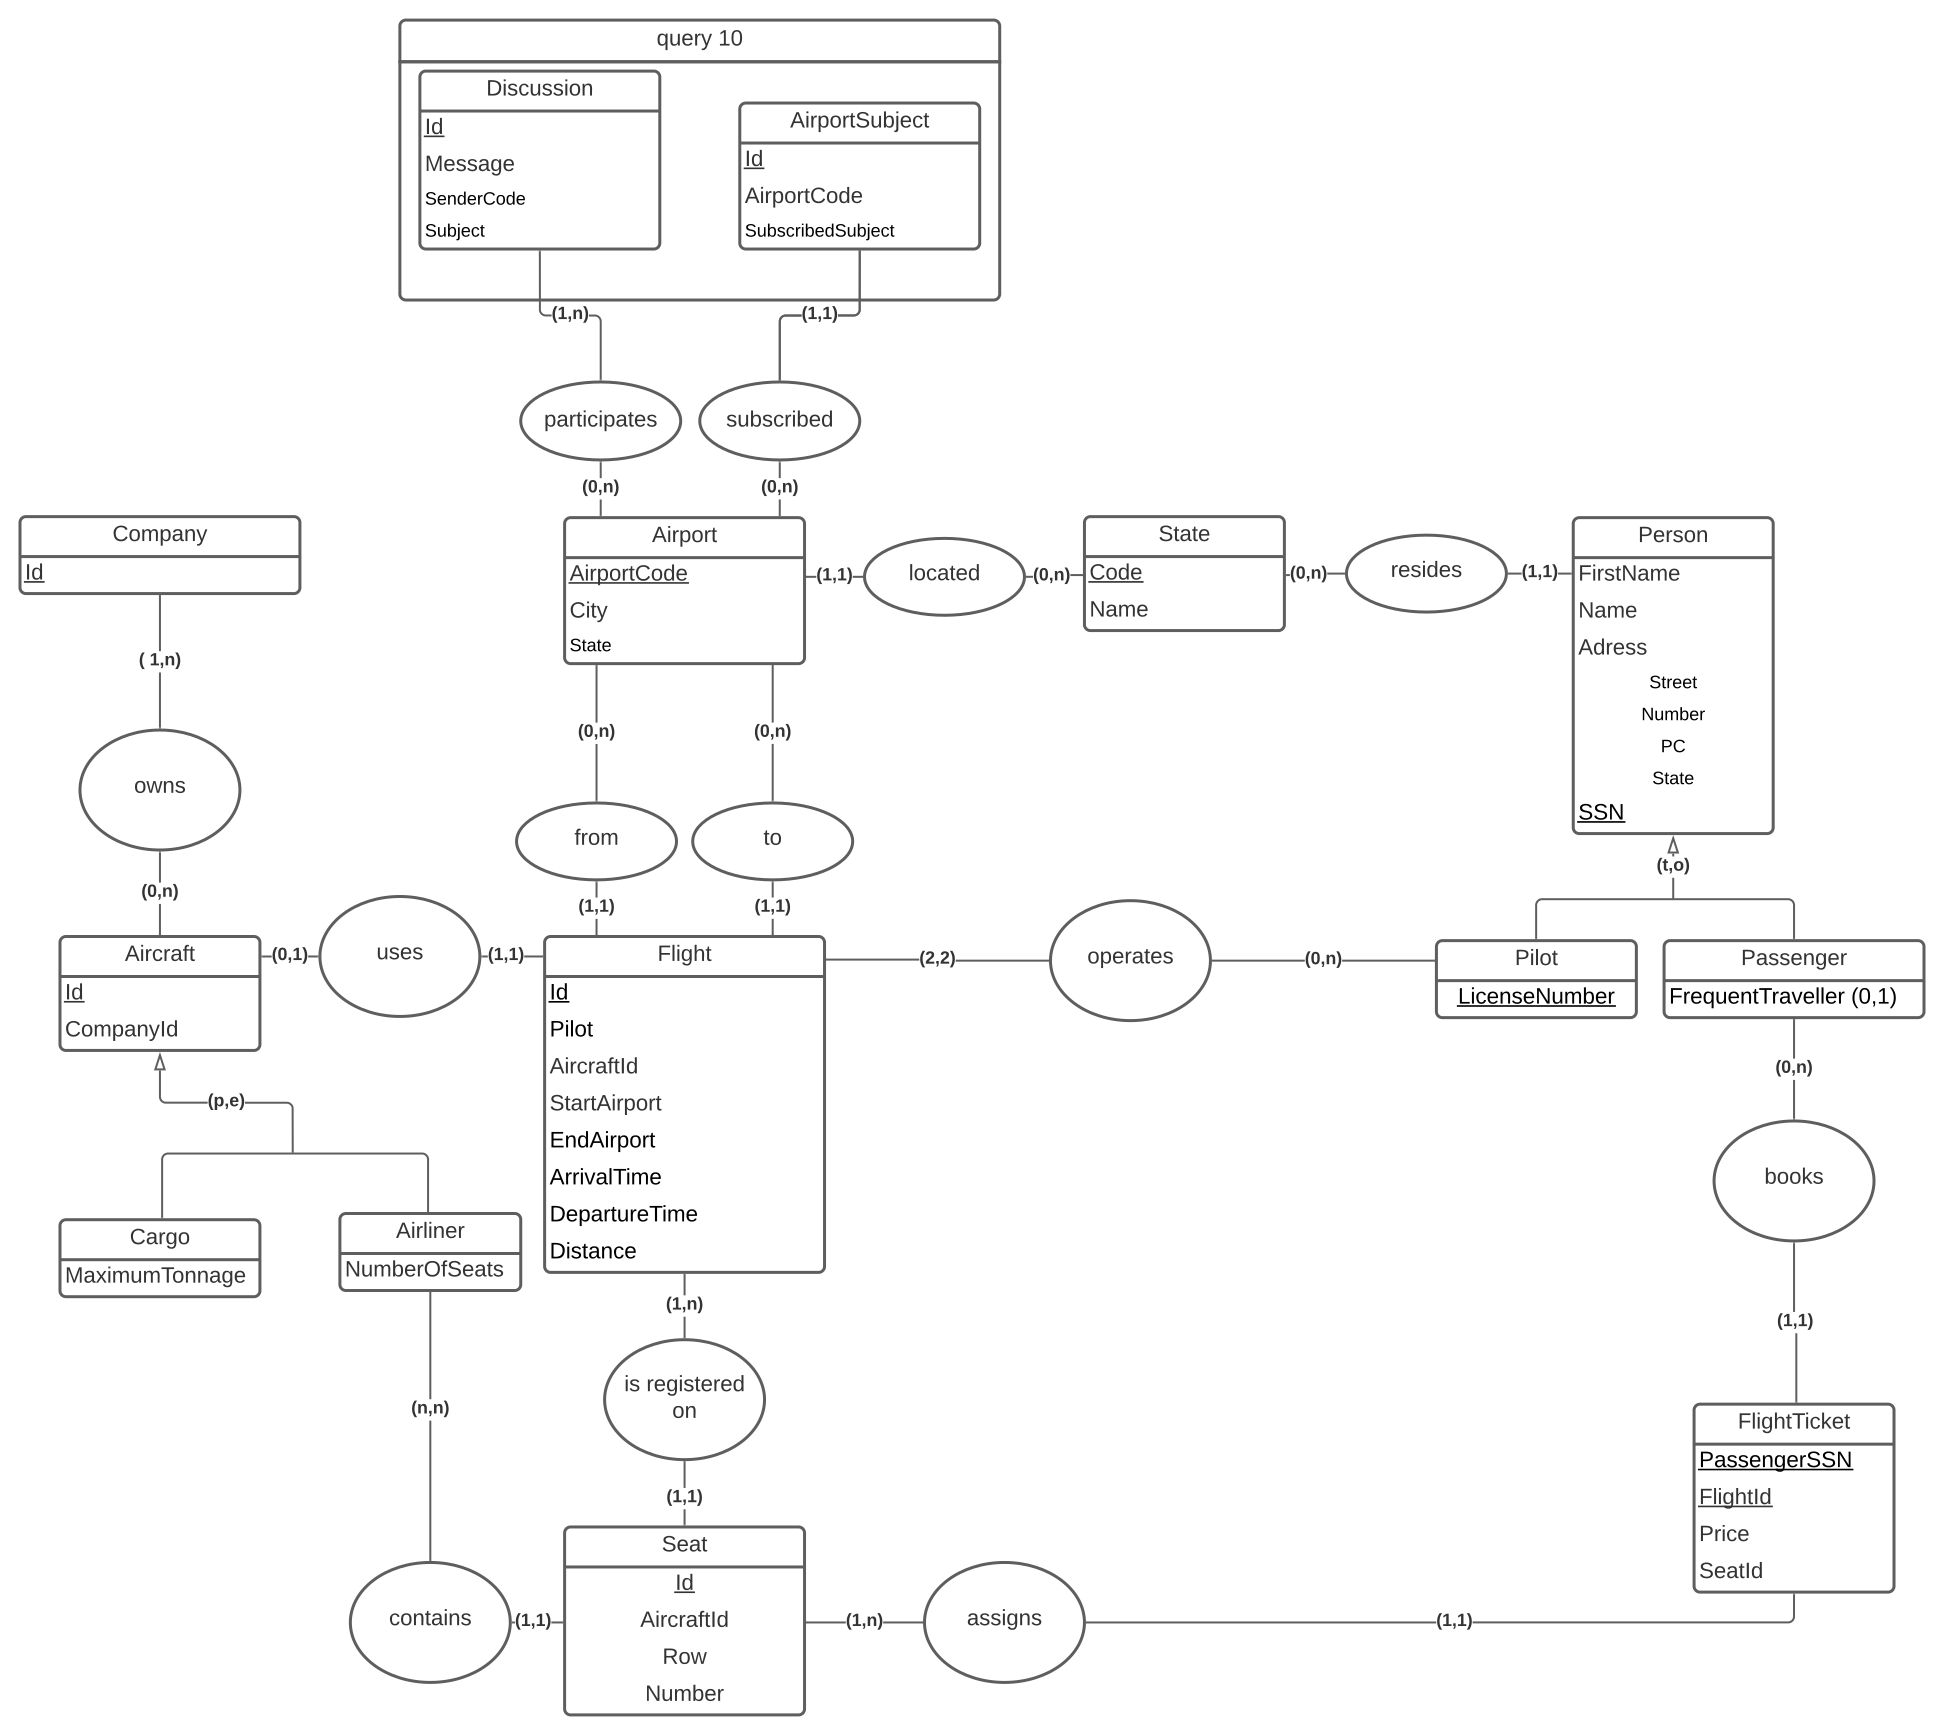
\includegraphics[width=\textwidth]{image/erd.png}
    \caption{Diagramme entité-association partie 1 corrigé}
    \label{fig:diag_p1_correction}
\end{figure}

\newpage

\subsection{Comparaison entre le modèle de la phase 1 et le modèle corrigé}

\begin{itemize}
    \item meilleure lisibilité sur la figure \ref{fig:diag_p1}
    \item pas de table Etat dans la figure \ref{fig:diag_p1} donc, perte de précision et risque de confusion car si l'état est encodé sous forme de code chez le passager et sous son nom complet chez l'aéroport les deux ne seront pas égaux

    \item "pilote operates" dans la figure \ref{fig:diag_p1} 0,1 vol faux, car le pilote peut être relié à plusieurs vols dans la database comme indiqué sur la figure \ref{fig:diag_correction} (0,n)
    \item un vol est opéré par un pilote et un copilote : cette possibilité est exclue par la figure \ref{fig:diag_correction}
    \item dans la figure \ref{fig:diag_p1} la clef du siège est composée de (aricraftid, row, number) alors que dans la figure \ref{fig:diag_correction} un id unique lui est attribué ce qui rend la manipulation des données plus facile.
    \item flight pourrait être une entité faible comme dans la figure  \ref{fig:diag_correction} car elle n'existe qu'à condition qu'elle soit reliée à un pilote
    \item réservation pourrait être une entité faible comme dans la figure \ref{fig:diag_correction} car elle n'existe qu'à condition qu'elle soit reliée à un avion
    \item seat pourrait être une entité faible comme dans la figure \ref{fig:diag_correction} car elle n'existe qu'à condition qu'elle soit reliée à un avion
    \item la relation P,e entre avion, avion de ligne et avions de fret dans la figure \ref{fig:diag_correction} permet de prendre en compte les avions de type autres alors que dans la figure \ref{fig:diag_p1}, seuls les avions de fret et de ligne étaient pris en compte
\end{itemize}

\newpage
\section{Traduction relationnelle}
\begin{itemize}
    \item Company(\underline{Id})
    \newline
    \item Aircraft(\underline{Id}, CompanyId, MaximumTonnage, NumberOfSeats)
    \subitem Aircraft.CompanyId ref Company.Id
    \newline

    \item State(\underline{Code}, Name)
    \newline

    \item Airport(\underline{AirportCode}, City, State)
    \subitem Airport.State ref State.Code
    \newline

    \textbf{Requête 10 uniquement}
    \hline
    \newline

    \item Discussion(\underline{Id}, Message, SenderCode, Subject)
    \subitem Discussion.SenderCode ref Airport.Code
    \newline

    \item AirportSubject(\underline{Id}, AirportCode, SubscribedSubject)
    \subitem AirportSubject.AirportCode ref Airport.Code
    \newline
    \hline
    \textbf{Fin de la requête 10}
    \newline

    \item Flight(\underline{Id}, AircraftId, StartAirport, EndAirport, ArrivalTime, DepartureTime, Distance)
    \subitem Flight.AircraftId ref Aircraft.Id
    \subitem Flight.StartAirport ref Airport.AirportCode
    \subitem Flight.EndAirport ref Airport.AirportCode
    \newline
    \subitem Contrainte :
    \subsubitem - StartAiport doit être différent de EndAirport
    \subsubitem - DepartureTime (moment de départ) < ArrivalTime (moment d'arrivée)
    \subsubitem - Distance > 0
    \newline

    \item Person(\underline{SSN}, FirstName, Name, AdressStreet, AdressNumber, AdressPC, AdressState, \underline{LicenseNumber}, FrequentTraveller)
    \subitem Person.AdressState ref State.Code
    \newline

    \item FlightTicket(\underline{PassengerSSN, FlightId}, Price, SeatId)
    \subitem FlightTicket.PassengerSSN ref Person.SSN
    \subitem FlightTicket.FlightId ref Flight.Id
    \subitem FlightTicket.SeatId ref Seat.Id
    \newline

    \item Seat(\underline{AircraftId, Row, Number}, PassengerSSN)
    \subitem Seat.AircraftId ref Aircraft.Id
    \subitem Seat.PassengerSSN ref Person.Id

\end{itemize}




\section{Justification}
Un vol est opéré par 2 pilotes, un capitaine et un copilote.
\newline
Le but d'ATASCO est d'aider les compagnies dans leur activité, une compagnie doit posséder un avion minimum pour être enregistrée.


Beaucoup de requêtes n'ont pas de traduction en algèbre relationnel, calcul tuple car elles utilisent des fonctions qui ne sont pas (simplement) traduisible dans ce formalisme t.q. count, avg, window function, etc.
\newpage

\section{Requêtes}
\subsection{Requête 1}
\subsubsection{SQL}
\begin{verbatim}
select count(vol.id)
from vol,
     aviondefret
where vol.avionid = aviondefret.id;
\end{verbatim}

\newpage

\subsection{Requête 2}

\subsubsection{SQL}
\begin{verbatim}
select pilote.id
from pilote,
     réservation
where réservation.voyageurid = pilote.id;
\end{verbatim}
\subsubsection{Algèbre relationnel}
\[ \pi_{pilote.id}[\sigma_{reservation.voyageurid=pilote.id}(pilote, reservation)]\]
\subsubsection{Calcul tuple}
\[\{p.piloteid\; | \;pilote(p) \wedge \exists l(reservation(l) \wedge l.voyageurid=p.id )\}\]
\newpage
\subsection{Requête 3}
\subsubsection{SQL}
\begin{verbatim}
with volPassager as (select count(voyageurid) as nombredepassager, réservation.volid
                     from réservation
                     group by réservation.volid
                     order by nombredepassager desc)

select volPassager.volid
from volPassager
where volPassager.nombredepassager = (select max(volPassager.nombredepassager) from volPassager);
\end{verbatim}
\newpage

\subsection{Requête 4}
\subsubsection{SQL}
\begin{lstlisting}
select vol.piloteid
from vol
except
select vol.piloteid
from vol,
     aviondefret
where vol.avionid = aviondefret.id;

\end{lstlisting}

---------------------------------------------

Si la base de données contient d'autres types d'avions que ceux de ligne ou fret:

\begin{lstlisting}

select vol.piloteid
from vol,
     aviondeligne
where vol.avionid = aviondeligne.id
except
select vol.piloteid
from vol,
     aviondefret
where vol.avionid = aviondefret.id;

\end{lstlisting}
\subsubsection{Algèbre relationnel}
\[piloteslignes(piloteid) \xleftarrow{} \{\pi_{piloteid} [vol - \sigma_{avionid=aviondefret.id}(vol, aviondefret)]\} \]
\subsubsection{Calcul tuple}
%\[\{\ v.piloteid\; | \;vol(v) \wedge  \exists a ( aviondeligne(a) \wedge v.avionid = a.id ) \wedge \lnot \exists f (aviondefret(f) \wedge  f.id = v.avionid) \}\]
\[\{\ p.piloteid\; | \;pilote(p) \wedge  \forall v\;vol(v) \xrightarrow{} ( p.id = v.piloteid \wedge \lnot \exists a(aviondefret(a) \wedge v.avionid = a.id)) \}\]
\newline
\newpage

\subsection{Requête 5}
\subsubsection{SQL}
\begin{verbatim}
select avg(distance), vol.heuredépart::date
from vol
where vol.avionid in (
    select avion.id
    from avion
    where avion.compagnieid in (
        select company.id
        from company
        where nom = 'ADVANCED AIR, LLC'
    )
)
group by vol.heuredépart::date
union
select avg(distance), vol.heuredépart::date
from vol
where vol.avionid in (
    select avion.id
    from avion
    where avion.compagnieid in (
        select company.id
        from company
        where nom = 'ABX Air Inc'
    )
)
group by vol.heuredépart::date;
\end{verbatim}
\newpage


\subsection{Requête 6}
\subsubsection{SQL}
\begin{verbatim}
select distinct aller.id as volAller,
                aller.heuredépart::time,
                retour.id as volRetour,
                retour.heuredépart::time
from vol as aller,
     vol as retour
where aller.heuredépart::time > '07:00:00'
  and aller.heuredépart::date = retour.heuredépart::date
  and retour.heuredépart >= aller.heurearrivée + '07:00:00'
  and aller.aéroportarrivéecode = retour.aéroportdépartcode
  and aller.aéroportdépartcode = retour.aéroportarrivéecode
  and aller.avionid in (select aviondeligne.id from aviondeligne)
  and retour.avionid in (select aviondeligne.id from aviondeligne);
\end{verbatim}
\newpage

\subsection{Requête 7}
\subsubsection{SQL}
\begin{verbatim}
select avg(companyidpassager.nombredepassager), company.nom
from company
         join(
    select avion.compagnieid, avionpassager.nombredepassager
    from avion
             join (
        select vol.avionid, passagervol.nombredepassager
        from vol
                 join (
            select count(réservation.voyageurid) as nombredepassager, réservation.volid
            from réservation
            group by réservation.volid
            having count(réservation.voyageurid) < 20
        ) as passagervol
                      on passagervol.volid = vol.id
    ) as avionpassager
                  on avion.id = avionpassager.avionid
) as companyidpassager
             on company.id = companyidpassager.compagnieid
group by company.nom;

\end{verbatim}


\newpage

\subsection{Requête 8}
\subsubsection{SQL}
\begin{verbatim}
with volsEnchainés as (
    select v.piloteid,
           v.heuredépart::date,
           (dense_rank() over (order by v.heuredépart::date) -
            row_number() over (partition by v.piloteid order by v.heuredépart::date)) as diffId
    from (
             select vol.piloteid,
                    vol.heuredépart::date,
                    lag(vol.heuredépart::date)
                    over (partition by vol.piloteid order by vol.heuredépart::date) as heuredépartPrécédent
             from vol) v
    where v.heuredépartPrécédent is NULL or v.heuredépart > v.heuredépartPrécédent
    order by v.piloteid, v.heuredépart::date
)

select max(vE.jours) as joursConsécutif, vE.piloteid
from (
         select count(volsEnchainés.diffId) as jours, volsEnchainés.piloteid
         from volsEnchainés
         group by volsEnchainés.piloteid, volsEnchainés.diffId
     ) vE
group by vE.piloteid
order by joursConsécutif desc;
\end{verbatim}

\begin{figure}[H]
\begin{center}
    \begin{tabular}{|c|c|c|c|c|}
        \hline
        Pilote & Date & IdInterne & Id & Îlots($\Delta$Id)\\

        \hline
        45d2a577-3734-4241-91eb-d789d78d18a4 & 12-05-22 & 1 & 3 & 2 \\
        & 13-05-22 & 2 & 4 & 2\\
        & 14-05-22 & 3 & 5 & 2\\
        \hline
        24e508fd-30d0-4172-bc4c-5cc6a789197f & 10-05-22 & 1 & 1 & 0 \\
        & 11-05-22 & 2 & 2 & 0 \\
        & 13-05-22 & 3 & 4 & 1 \\
        \hline
    \end{tabular}
\end{center}
    \caption{Exemple de table intermédiaire illustrant la résolution de la requête 8}
    \label{fig:requete8}
\end{figure}


\newpage

\subsection{Requête 9}
\subsubsection{SQL}

\begin{verbatim}
create table if not exists pilote_expert
(
    id        uuid primary key,
    date      date,
    estExpert boolean
);


create temp table temp_pilote_expert
(
    id_expert   varchar(128),
    date        varchar(128)
);

copy temp_pilote_expert (id_expert, date)
    from 'fichier.csv'
    delimiter ','
    header csv;


insert into pilote_expert(id, date, estExpert)
select split_part(temp_pilote_expert.id_expert, '--', 2)::uuid,
       temp_pilote_expert.date::timestamp,
       case -- switch comme en C++
           when split_part(temp_pilote_expert.id_expert, '--', 1) = 'existing-expert' then true
           when split_part(temp_pilote_expert.id_expert, '--', 1) = 'new-expert' then false
           else false
           end
from temp_pilote_expert
where not exists( -- verification que l'on n'insere pas une ligne deja présente
        select pilote_expert.id
        from pilote_expert
        where id = split_part(temp_pilote_expert.id_expert, '--', 2)::uuid
    );

\end{verbatim}
\newpage

\subsection{Requête 10}
\subsubsection{SQL}

%\begin{lstlisting}[language=SQL]
\begin{verbatim}
create table if not exists aéroportsujets
(
    id           uuid default uuid_generate_v4() primary key not null,
    aéroportCode varchar(8)                                  not null
        constraint fk_aéroportCode
            references aéroport,
    sujetAbonné  text                                        not null
);


insert into aéroportsujets(id, aéroportCode, sujetAbonné)
values (default, 'AKN', 'mobilité');
insert into aéroportsujets(id, aéroportCode, sujetAbonné)
values (default, 'AKN', 'économie');
insert into aéroportsujets(id, aéroportCode, sujetAbonné)
values (default, 'AKN', 'écologie');


create table if not exists discussion
(
    id             uuid default uuid_generate_v4() primary key not null,
    message        text                                        not null,
    expéditeurCode varchar(8)                                  not null
        constraint fk_expéditeurCode
            references aéroport,
    sujet          text                                        not null
);

\end{verbatim}

\section{Référence} \label{sec:ref}

\begin{itemize}
    \item Wikipédia modèle entité-association "\url{https://fr.wikipedia.org/wiki/Mod%C3%A8le_entit%C3%A9-association}" vu le 05/05/2022
\end{itemize}

\end{document}
